\section{Results}
\label{sec:results}

\subsection{Stationary data}

The characteristic lift force data for a stationary body ($C_y$) as a function of incident angle $\theta$ obtained using flow simulations are shown in figure \ref{cy ploynomial}(a). They agree well with the low \reynoldsnumber\ data presented in \citet{Joly2012}.

However, there are several differences that can be observed when the low \reynoldsnumber\ data are compared with the $7^{th}$ order polynomial curve at $\reynoldsnumber=22300$ shown in figure \ref{cy ploynomial}(b). The peak value of $C_y$ is  significantly lower at $\reynoldsnumber=165$ ($C_y=0.05$ at $4^\circ$) in comparison with $\reynoldsnumber=22300$ ($C_y=0.57$ at $13^\circ$) . The inflection point present around $8^\circ$ for $\reynoldsnumber=22300$ is not observed at $\reynoldsnumber=165$. This agrees with the findings of \cite{Luo2003}. 

It was concluded by \cite{Luo2003} that hysteresis in the system response occurs due to the inflection point in the $C_y$ curve. Therefore hysteresis is not expected at $\reynoldsnumber=165$.

The range of incident flow angles where $C_y$ remains positive is narrow at $\reynoldsnumber=165$ ($0^\circ <\theta \leq$ $6^\circ$) compared to $\reynoldsnumber=22300$ ($0^\circ <\theta \leq 15^\circ$). This feature is what sustains galloping. Power is only transferred from the fluid to the supporting structure within this range of incident angles because fluid forces are acting in the direction of travel of the oscillating cylinder, as demonstrated by equation \ref{power_alt}. Incident angles beyond this range actually suppress the galloping and power goes in the opposite direction, i.e; form body to fluid. Therefore due to the overall smaller $C_y$ and narrow range of angles where $C_y$ is positive for $\reynoldsnumber=165$ compared to $\reynoldsnumber=22300$, it is expected that power output at $\reynoldsnumber=165$ is significantly lower than at $\reynoldsnumber=22300$. 

\input{../figure/uncollapsed_data}

\subsection{Displacement, velocity and power output as a function of reduced velocity}

 The quasi-steady analysis data reveal that the displacement amplitude grows with increasing $U^*$. This is shown for both the high and low \reynoldsnumber\ cases in figures \ref{fig:uncollapsed_data} (a) and (b). The onset of galloping is delayed with increasing damping ratio $\zeta$ for both high and low Reynolds numbers. This echos the findings of previous studies by \cite{Parkinson1964} and \cite{Barrero-Gil2010a}. Hysteresis could be observed for the case with a higher Reynolds number. Different solutions could be obtained by manipulating the initial conditions (initial displacement) of the system. The upper branch was obtained by giving an initial displacement which was higher than the expected amplitude while the lower branch was obtained by providing a lower initial displacement than the expected amplitude. Although theory shows a possible third state, it is an unstable branch and as such it could not be achieved numerically. This was also observed by \cite{Vio2007}.   

\subsubsection*{Power vs $U^*$}
 
 The mean power grows, peaks and then slightly reduces as the reduced velocity $U^*$ is increased. This is shown in figure \ref{fig:uncollapsed_data}(e) and (f) for each value of $\zeta$. The value of  \ustar\ at which the peak power occurs increases with $\zeta$. However, the magnitude of the peaks remain constant for all the values of $\zeta$. \citet{Barrero-Gil2010a} also observed a similar behaviour. The higher Reynolds number case clearly shows hysteresis in the power data. The range of hysteresis increases with increasing $\zeta$.

Unlike VIV, which is a resonant-type phenomenon, the quasi-steady system describing galloping has no strongly preferred frequency. Although the onset of galloping and the value of \ustar\ where peak power occurs varies with the damping ratio $\zeta$, the power extracted remains almost constant for values of \ustar\ beyond that where the peak power occurs. 

The efficiency of the system can be defined as the ratio of the time average power output to $P_{mean}=\rho U^3\frac{D}{2}$, the kinetic energy in the fluid approaching the body. A similar definition was given in \citet{Barrero-Gil2010a}). The current results show that the system has a peak efficiency of $0.26\%$  for $\reynoldsnumber=165$ and $6.7\%$ for $\reynoldsnumber=22300$. The peak efficiency reported in \citet{Barrero-Gil2010a} for \JL{KASUN: include the Re from Barrero-Gil} is approximately $5\%$ less than the current result. This difference is due to \cite{Barrero-Gil2010a} using a $3^{rd}$ order polynomial as the interpolating polynomial which under predicts the forcing at values of $\theta$ where the maximum force occurs as compared to the $7^{th}$ order polynomial used in this study.   
 
\JL{Up to here 12.20pm}

 \subsection{Galloping response and natural frequency}
 
 Now the oscillator equation Eq.\eqref{final_equation_motion} is considered from a power perspective. The shedding forces can be neglected because the net effect is negligible as system oscillates at natural frequency which is far from shedding frequency, for the cases that exhibit galloping. It is obvious that the forcing term on LHS of the equation is only dependent on transverse velocity($\dot{y}$) which is essentially the input power of the system. On the RHS, the mechanical damping or system damping is the only term that takes out power at any instant. This could be expressed as the product of the damping force and the velocity ($P_d$). The inertia and the stiffness terms governs the frequency of the system but the forces associated with those terms are conservative forces (i.e there is zero net energy in or out of the system when averaged over a period). Therefore the system is governed by the transverse velocity rather than the natural frequency.
 

 Using $U^*$ and $\zeta$ assumes that the system has a preferred frequency because the scale with the natural frequency of the system. The effect of fixing $\zeta$ and increasing $U^*$ actually decreases the damping constant for a fixed free-stream velocity. ($U^*=\frac{U}{f \times D}$, $\zeta= \frac{c}{2 m \omega_n}$ ). Both these effects leads to the multiple lines that are horizontally transpose when $\zeta$ is increased (Fig.\ref{fig:uncollapsed_data} (e) and (f)). Therefore the effect of $\zeta$ essentially scales up the damping coefficient for a fixed $U^*$.
 
 The data presented in Fig.\ref{fig:uncollapsed_data} for various damping ratios, $\zeta$, can be collapsed into a single line for a for a particular force characteristic curve (i.e $C_y$ vs $\theta$ curve). These collapsed curves were  obtained for the velocity amplitude  and power by plotting as functions of as a function of  the non dimensionalised  damping constant $\frac{c}{\rho\mathcal{A}U}$ 
(Fig \ref{fig:collpased_data} (a),(b),(c) and (d)).  This further emphasizes that the galloping system is not frequency dependent. It is possible to obtain a similar power output at different values of \ustar when the damping constant, $\frac{c}{\rho\mathcal{A}U}$, is kept fixed. An example of this case, as shown in Fig.\ref{fig:time_hostory_velocity_same_power}, clearly show that this is a result of similar velocity amplitudes between cases if one were to disregard the high frequencies due to shedding. As mentioned earlier, it is the transverse velocity that determines the energy provided by the fluid forcing and the mechanical damping.

\begin{figure}
  \setlength{\unitlength}{\textwidth}
       
        \begin{picture}(1,0.52)

      % % % Parkinson Data 
      \put(0.025,0.27){\includegraphics[width=0.5\unitlength]{../FnP/gnuplot/velocity_amp_collapsed_parkinson.eps}}
      \put(0.495,0.27){\includegraphics[width=0.5\unitlength]{../FnP/gnuplot/velocity_amp_collapsed_re165.eps}}
      
      \put(0.025,0.02){\includegraphics[width=0.5\unitlength]{../FnP/gnuplot/mean_power_collapsed_parkinson.eps}}
      \put(0.495,0.02){\includegraphics[width=0.5\unitlength]{../FnP/gnuplot/mean_power_collapsed_re_165.eps}}
      
      
      \put(0.23,0.00){ $c\rho\mathcal{A}U$}
      \put(0.73,0.00){ $c\rho\mathcal{A}U$}
      
      \put(0.01,0.405){$\frac{V}{D}$}
      
      \put(0,0.13){$\frac{P_{m}}{\rho \mathcal{A}U^3 }$}
      \put(0.085,0.475){\small(a)}
      \put(0.555,0.475){\small(b)}
      \put(0.085,0.225){\small(c)}
      \put(0.555,0.225){\small(d)}
      
    \end{picture}

  \caption{Velocity amplitude and mean power as functions of the damping factor. Data presented in (a) and (c)  were calculated using input data at $Re=22300$ obtained by \cite{Parkinson1964} at three different damping ratios: $\zeta=0.0125$ (\ding{83}), $\zeta=0.015$ (\ding{116}) and $\zeta=0.0175$ (\ding{108}). Data presented in (b)and (d)  were obtained using input data at $Re=165$ at three different damping ratios: $\zeta=0.075$ ($\times$), $\zeta=0.1$ (\ding{117}) and $\zeta=0.15$ (+). The collapsed data implies that there is no frequency selection and the tuning parameter of the mechanical side of the system is the damping constant to obtain an optimum power output.}
    \label{fig:collpased_data}
\end{figure}

\ %vspace{10cm}

 
\begin{figure}
  \setlength{\unitlength}{\textwidth}
  \begin{picture}(1,0.3)(0,0.8)
    % % %90
    \put(0.025,0.83){\includegraphics[width=0.5\unitlength]{../FnP/gnuplot/vel_time_history_60_0.075.eps}}
    \put(0.495,0.83){\includegraphics[width=0.5\unitlength]{../FnP/gnuplot/vel_time_history_165_0.175.eps}}
    
    \put(0.03,0.95){ $\frac{V}{D}$} 	
    % \put(0.56,1.02){ $\frac{V}{D}$}
 	
    \put(0.25,0.805){ $\frac{tU}{D}$} 	
    \put(0.73,0.805){ $\frac{tU}{D}$}

    \put(0.095,1.03){(a)}
    \put(0.565,1.03){(b)}

  \end{picture}

  \caption{Time histories of velocity at two different $\zeta$ and $U^*$ which produce the same mean power ($1.2\times10^{-3}$). Data presented in (a) are at $\ustar=60$, $\zeta=0.075$ and (b) are at $\ustar=165$, $\zeta=0.175$. Both data sets were obtained using Quasi-steady state assumption using input $C_y$ parameters at $Re=165$. Shedding is evident in both signals as a high frequency fluctuation but the amplitude of the slower fluctuations remains constant in both cases.}
    \label{fig:time_hostory_velocity_same_power}
\end{figure}

 


 
 Power could be expressed as the product of force and velocity. Therefore the transferred power form fluid-to-body could be expressed as $P_t=F_y\dot{y}$. Similarly the dissipated power due to the mechanical damping could be expressed as $P_d=(c\dot{y})\dot{y}$. The time average of these two quantities should be equal due to energy conservation, provided that the mechanical friction is neglected . Analysing the  time histories of $P_t $ and $P_d$ at key regions (Fig.\ref{fig:regions_1}) on the mean power vs $U^*$ provides a detailed explanation for the variation of the output power when the reduced velocity is increased. The key regions consists of region 1 where the $P_{mean}$ increases with \ustar, region 2 where $P_{mean}$ becomes maximum and region 3 where $P_{mean}$ decreases with \ustar. It has been established earlier that the damping factor is a function of $U^*$. Therefore it could be derived that $U^*$ is inversely proportional to damping coefficient. Hence the damping coefficient reduces when you move from region 1 to 3. Fig \ref{fig:lift_curves} (a) shows that $C_y$ and therefore instantaneous force rises until $4^\circ$ where it peaks and then falls and at around $6^\circ$ becomes negative. The maximum amount of power that could be transferred occurs near the peak region. At the region where the instantaneous force becomes negative it will be opposing the velocity $\dot{y}$. Data at $\zeta=0.1$, $m^*=40$ and \reynoldsnumber=165 (Fig.\ref{fig:power_time_histories}) are analysed as and example.  

\begin{figure}[h!]
\centering
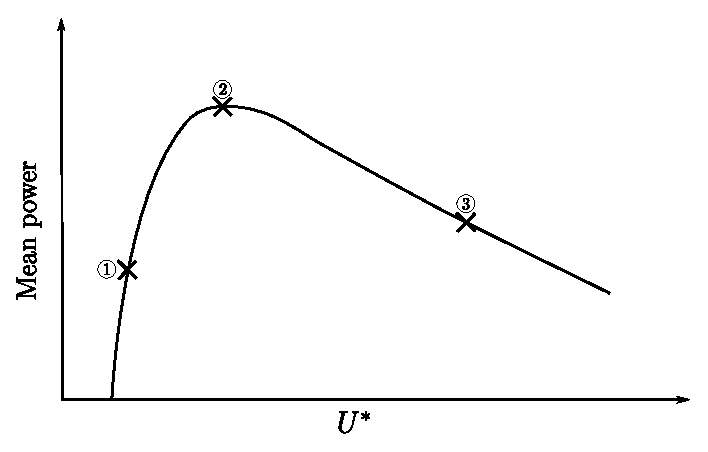
\includegraphics[width=0.5\textwidth]{../FnP/sketch_1}
\caption{ Three key regions taken into account to analyse the time histories of power in a typical mean power vs. $U^*$ curve at $Re=165$. In region 1, high damping suppresses oscillation, hence the power output is low. In region 2, the damping is close to the optimum for power transfer. In region 3, the low damping means little energy is extracted from the fluid.}
\label{fig:regions_1}
\end{figure}

 
 
 
 At region 1 where $U^*=90$ the damping constant is high and a clear sinusoidal signal could be observed for both $P_d$ and $P_t$ in Fig.\ref{fig:power_time_histories} (a). Fig.\ref{fig:power_time_histories} (d) and (g) shows that $\theta$ is in line or in phase with $F_y$.  The velocity amplitude in this case is small and the equivalent incident angle within the range where the hydrodynamic force increases with the incident angle (i.e. $0<\theta \leq 4^\circ$ in Fig.\ref{fig:lift_curves} (a)) Hence both $P_d$ and $P_t$ becomes sinusoidal. In this case, power output is limited by the low fluid forces present at low incident angles. In other words damping is significantly high and extracts a lot of power that the velocity amplitude could not grow where the forcing  is significant to produce high level of power.   
 
 
  At region 3 ($U^*= 400$) `$c$' is low in comparison with region 1 and 2 which leads to a low mean power output. Fig.\ref{fig:power_time_histories} (c) shows that $P_t$ becomes negative over some portion of the cycle. This is caused by te high velocity amplitude leads to the equivalent incident angle $\theta$, in this case to exceed the range where $C_y$ is positive (i.e. $0<\theta<6^\circ$ in Fig.\ref{cy ploynomial} (a)). In this portion of the cycle the hydrodynamic force actually opposes the direction of travel and power is transferred from the structure to the fluid during those times. From and energy perspective, the mechanical damping is not sufficient to remover the energy transferred from the fluid to the structure during other times of the cycle because $\frac{c}{\rho\mathcal{A}U}$ is substantially low. Therefore this excess energy is transferred back to the fluid as depicted by the negative region of $P_d$ in Fig.\ref{fig:power_time_histories} (c) 
 

At region 2 ($U^*=165$). $P_t$ is not a pure sinusoidal signal. However, the  signal remains periodic. From the time history graph of $P_t$, two `peaks' are present in a single half cycle (Fig \ref{fig:power_time_histories} (b)). In this case, the velocity amplitude actually exceeds the equivalent incident angle where the hydrodynamic forces peaks (i.e. $\theta=4^\circ$ in \ref{cy ploynomial} (a)). The dips in $P_d$ between the two peaks approximately correspond to the time where the transverse velocity is higher than 0.07 and $F_y$ is decreasing with increasing transverse velocity. The mean power output is at its maximum. This is due to the fact that this region is a best compromise between region 1 and 3. The damping is substantially high to obtain a high power output while not too high to allow the induced angle of attack to enter the region where the forcing opposes the direction of travel. 


 
  
\input{../figure/time_histories}


\subsection{Effect of $m^*$}

 \begin{figure}
\setlength{\unitlength}{\textwidth}

  \begin{picture}(1,0.35)(0,0.75)
    
  \put(0.15,0.76){\includegraphics[width=0.7\unitlength]{../FnP/gnuplot/mean_power_collapsed_mstar.eps}}         
      
      
   
 	\put(0.11,0.95){\large $\frac{P_{m}}{\rho \mathcal{A}U^3 }$} 	

 	
 	 	\put(0.45,0.75){ $c\rho\mathcal{A}U$} 	
 	 

     

  \end{picture}

  \caption{Mean power as a function of damping factor. Data are presented at $m^*=10$ (\ding{108}), $m^*=20$ (\ding{83}), $m^*=40$ (\ding{115}), $m^*=60$ (+) at Re 165 and $\zeta=0.1$. A reduction of maximum mean power can be observed when $m^*<40$. For $m^*>40$, the maximum power is essentially independent of $m^*$.}
    \label{fig:m_star_collapsed}
\end{figure}
 \begin{figure}
  \setlength{\unitlength}{\textwidth}
\fbox{
        \begin{picture}(1,0.3)(0.0,0.45)

      % % % Parkinson Data 
      \put(0.025,0.5){\includegraphics[width=0.5\unitlength]{../FnP/gnuplot/mean_power_collapsed_mstar_175.eps}}      \put(0.495,0.5){\includegraphics[width=0.5\unitlength]{../FnP/gnuplot/mean_power_collapsed_parkinson_10.eps}}
      
      \put(0.23,0.48){ $\displaystyle\frac{c}{\rho\mathcal{A}U}$}
      \put(0.73,0.48){ $\displaystyle\frac{c}{\rho\mathcal{A}U}$}
          
      \put(0.0,0.63){\large$\frac{P_{m}}{\rho \mathcal{A}U^3 }$}
      
      \put(0.085,0.709){\small(a)}
      \put(0.555,0.709){\small(b)}
     
      
    \end{picture}
}
  \caption{}
    \label{fig:collpased_data}
\end{figure}

\ %vspace{10cm}


The maximum mean power at different $m^*$ (Fig.\ref{fig:m_star_collapsed}(a)) was constant for $m^*>30$ in the low \reynoldsnumber\ case. However, at $m^* \leq 30$, the power output reduces with reducing $m^*$ across the parameter range. However, when the sinusoidal forcing function in Eq.\ref{equationofmotion} which cater for the vortex shedding was disregarded, the reduction in power could not be observed Fig.\ref{fig:m_star_collapsed}(b). The suppression of galloping response at low $m^*$ due to the presence of vortex shedding has previously been observed by \cite{Joly2012}. This is a non-linear interaction between the forcing that drives the galloping excitation and the forcing as a result of vortex shedding. The forcing associated with vortex  shedding is significantly larger and at a higher frequency than the forcing that drives galloping. Systems with low $m^*$ do not have enough inertia to fully sustain the galloping excitation over the longer period.

At \reynoldsnumber=22300 power output started to increase for cases with $m^*<50$. The overall mean power tend to increase  as the $m^*$ was decreased when $U^*$ was kept constant (Fig\ref{fig:mstarcollapsed_parkinson} (a)). The same effect was observed when $U^*$ was increased keeping $m^*$ constant (\ref{fig:mstarcollapsed_parkinson} (b)). It should be noted that the influence of $U^*$ was observed only for low mass ratios.  The velocity time traces of example cases of both scenarios presented in Fig.\ref{time_hostory_mstar_mass} and \ref{time_history_mstar_ustar} shows that essentially the same phenomenon occurring in both cases whereby the velocity signal tend to shift from a sinusoidal signal towards a square wave. The corresponding displacement signal tend to become more like a triangular wave. When the inertia of the system reduces, the body can accelerate faster thus attaining higher velocities more rapidly and spend a higher proportion of the period at a high velocity. Higher velocities are favourable because they result in higher instantaneous hydrodynamic forcing and power output from mechanical damping. However, the velocity is limited by the characteristic of the hydrodynamics forcing which reaches a maximum and then decreases past an incident angle of of $13.21^{\circ}$ which correspond to a transverse velocity of $\frac{\dot{y}}{U}=0.235$.It is estimated that the efficiency limit i.e ($\ustar \rightarrow \infty$, $m^* \rightarrow 0$ and $\frac{c}{\rho U \mathcal{A}}=1.22$) will approach $13.5\%$ which corresponds to a square wave velocity signal with a velocity amplitude that results in maximum  hydrodynamic forcing. Physical systems may not realize the full potential due to practical limitations. Increasing $U^*$ effectively reduces the stiffness of the system and lengthen the period, thus again allowing a larger portion of the period to be at a high velocity which favours power output. For the case of fixing $U^*$ and decreasing $m^*$ in (Fig\ref{fig:mstarcollapsed_parkinson} (a)), the lengthening of the period is associated with the added mass which is kept constant at 3.5 being more dominant on the overall mass of the system when m* is reduced. 


  




\input{../figure/time_history_msar_mass}

\begin{figure}

  \setlength{\unitlength}{\textwidth}
  
 \begin{picture}(1,0.399)(0.01,0.77)
     % % % 90
     \put(0.03,1){\includegraphics[width=0.35\unitlength]{../FnP/gnuplot/vel_time_history_1164.eps}}   
     \put(0.36,1){\includegraphics[width=0.35\unitlength]{../FnP/gnuplot/vel_time_history_10.eps}}
     \put(0.68,1){\includegraphics[width=0.35\unitlength]{../FnP/gnuplot/vel_time_history_5.eps}}
         
     \put(0.03,0.82){\includegraphics[width=0.35\unitlength]{../FnP/gnuplot/dis_time_history_1164.eps}}   
     \put(0.36,0.82){\includegraphics[width=0.35\unitlength]{../FnP/gnuplot/dis_time_history_10.eps}}
     \put(0.68,0.82){\includegraphics[width=0.35\unitlength]{../FnP/gnuplot/dis_time_history_5.eps}}
     
 
     
     \put(0.55,0.79){$\displaystyle{\frac{tU}{D}}$}
     \put(0.2,0.79){$\displaystyle{\frac{tU}{D}}$}
     \put(0.85,0.79){$\displaystyle{\frac{tU}{D}}$}
     
      \put(0.02,1.07){$\displaystyle\frac{V}{D}$}
     \put(0.02,0.9){$\displaystyle\frac{A}{D}$}
 
     
     \put(0.08,0.9997){(a)}    
     \put(0.4,0.9997){(b)}    
     \put(0.72,0.9997){(c)}
     \put(0.08,0.8){(d)}    
     \put(0.4,0.8){(e)}    
     \put(0.72,0.8){(f)}
     
    
   \end{picture}


  \caption{Time histories of velocity. Data presented at \reynoldsnumber=22300, $m^*=10$ and $\frac{c}{\rho\mathcal{A}U}=9.3\times10^{-1}$ at three different reduced velocities: (a) $\ustar=75$, (b) $\ustar=175$ and (a) $\ustar=375$. As the mass ratio decreases the signal tend to transform from a sinusoidal towards a square signal due to the reduction in inertia.}
  
  \label{time_history_mstar_ustar}
\end{figure}





\input{../figure/qss_fsi}
 

\subsection{Comparison with FSI simulations}
 Similar trends were captured for both displacement and velocity amplitudes between QSS and FSI simulations (Fig. \ref{fig:FSI_QSS_compare}(a) and \ref{fig:FSI_QSS_compare}(b)). Quantitatively a large discrepancy (average of $30\%$) could be observed between QSS and FSI data. Therefore the power also becomes significantly low in FSI data (Fig.\ref{fig:FSI_QSS_compare} (c)). However, the FSI data (Fig.\ref{fig:FSI_QSS_compare} (c)) were able to produce the main the rise and the fall of mean power when $U^*$ was increased. The reasoning behind this fact is that galloping is weak at \reynoldsnumber$=165$  and therefore fluid damping has a significant effect. It was reported by \cite{Barrero-Gil2009} that galloping only starts to occur ar Re $\geq 159$. As power is a function of $(\dot{y})^2$ the error between QSS and FSI power is compounded.  
 

 

\section{Conclusion}
\label{sec:conc}

In this paper, the power transfer of a square body under aero elastic galloping is analysed by solving the quasi-steady state model equations through numerical integration. At higher $m^*$ ($m^8>30$ at lower \reynoldsnumber and $m^*> 50$ at high \reynoldsnumber) the power output of the system is not dependent on \ustar or natural frequency of the system, but controlled by the non-dimensionalised damping constant $\frac{c}{\rho U \mathcal{A}}$ . By analysing key regions of the power vs \ustar curve it could be concluded that in order to obtain an optimum power output, the damping constant ($\frac{c}{\rho\mathcal{A}U}$) should be high, but not excessive until it  to hinders the galloping from reaching induced angles of attack where the forcing is significant. The effect of mass ratio was could also be observed where at \reynoldsnumber=165. The peak efficiency was found out to be $0.26\%$ for \reynoldsnumber=165 and $6.7\%$ for \reynoldsnumber=22300  when $\frac{c}{\rho \mathcal{A}U}=0.314$ and $\frac{c}{\rho \mathcal{A}U}=1.04$ respectively. The mean power tend to decrease at $m^*<50$ which was found out to be an influence of vortex shedding. At \reynoldsnumber=22300 an opposite result could be observed where the mean power tend to increase with decreasing mass ratio as well as the mean power tend to increase with increasing $U^*$ at low mass ratios. When the mass ratio decreases, due to the lower inertia the velocity time trace tend to move from a sinusoidal signal towards a square signal where it sustains high velocities for longer periods of time which leads to a higher mean power output. The limit to peak efficiency was found out to be $13.5\%$ and occurs when $m^*\rightarrow 0$ and $\ustar \rightarrow \infty$ and $\frac{c}{\rho \mathcal{A}U}=1.22$ by analysing the data trend by lowering the $m^*$






 

 
 
 

 
 


 % % % % % % % % % % % % % % % % % % % % % % % % % % % % % % % % % % % % % % % % %

 
 
 
 
 
 
 
 
 
 
  
 
 
